%\documentstyle[epsf,twocolumn]{jarticle}       %LaTeX2e仕様
\documentclass[twocolumn]{jarticle}     %pLaTeX2e仕様(platex.exeの場合)
% \documentclass[onecolumn]{ujarticle}   %pLaTeX2e仕様(uplatex.exeの場合)
%%%%%%%%%%%%%%%%%%%%%%%%%%%%%%%%%%%%%%%%%%%%%%%%%%%%%%%%%%%%%%
%%
%%  基本バージョン
%%
%%%%%%%%%%%%%%%%%%%%%%%%%%%%%%%%%%%%%%%%%%%%%%%%%%%%%%%%%%%%%%%%
\setlength{\topmargin}{-45pt}
%\setlength{\oddsidemargin}{0cm}
\setlength{\oddsidemargin}{-7.5mm}
%\setlength{\evensidemargin}{0cm}
\setlength{\textheight}{24.1cm}
%setlength{\textheight}{25cm}
\setlength{\textwidth}{17.4cm}
%\setlength{\textwidth}{172mm}
\setlength{\columnsep}{11mm}

%\kanjiskip=.07zw plus.5pt minus.5pt


% 【節が変わるごとに (1.1)(1.2) … (2.1)(2.2) と数式番号をつけるとき】
%\makeatletter
%\renewcommand{\theequation}{%
%\thesection.\arabic{equation}} %\@addtoreset{equation}{section}
%\makeatother

%\renewcommand{\arraystretch}{0.95} 行間の設定
%%%%%%%%%%%%%%%%%%%%%%%%%%%%%%%%%%%%%%%%%%%%%%%%%%%%%%%%
%\usepackage{graphicx}   %pLaTeX2e仕様(\documentstyle ->\documentclass)
\usepackage[dvipdfmx]{graphicx}
\usepackage{subcaption}
\usepackage{multirow}
\usepackage{amsmath}
\usepackage{url}
\usepackage{ulem}
\usepackage{algorithm}
\usepackage{algorithmic}
\usepackage{listings} %,jlisting} %日本語のコメントアウトをする場合jlistingが必要
%ここからソースコードの表示に関する設定
\lstset{
  basicstyle={\ttfamily},
  identifierstyle={\small},
  commentstyle={\smallitshape},
  keywordstyle={\small\bfseries},
  ndkeywordstyle={\small},
  stringstyle={\small\ttfamily},
  frame={tb},
  breaklines=true,
  columns=[l]{fullflexible},
  numbers=left,
  xrightmargin=0zw,
  xleftmargin=3zw,
  numberstyle={\scriptsize},
  stepnumber=1,
  numbersep=1zw,
  lineskip=-0.5ex
}
\newcommand{\argmax}{\mathop{\rm arg~max}\limits}
\newcommand{\argmin}{\mathop{\rm arg~min}\limits}

%%%%%%%%%%%%%%%%%%%%%%%%%%%%%%%%%%%%%%%%%%%%%%%%%%%%%%%%
\begin{document}

	%bibtex用の設定
	%\bibliographystyle{ujarticle}

	\twocolumn[
		\noindent
		\hspace{1em}
		2020 年 12 月 25 日
		ゼミ資料
		\hfill
		B4 杉山 竜弥
		\vspace{2mm}

		\hrule
		\begin{center}
			{\Large \bf 進捗報告}
		\end{center}
		\hrule
		\vspace{9mm}
	]

\section{今週やったこと}
\begin{itemize}
  \item TDGAの実装
\end{itemize}

\section{エントロピーの定義の変更}

\begin{equation}
  H = \sum_{k \in \mathcal{P}} \sqrt{\mathrm{MSE}( \alpha_k, \bar{\alpha} )}
\end{equation}
標準偏差の和とした.

\section{トイ問題}
\begin{itemize}
  \item 個体は 3x3 のゼロ行列
  \item 適応度は各要素の総和
  \item 最小化問題
\end{itemize}

\section{実験設定}

\begin{table}[tb]
  \begin{center}
    \caption{GAの設定 ~~()は遺伝子座ごと}
    \begin{tabular}{|c|c|} \hline
      個体数 & 10 \\ \hline
      世代数 & 20 \\ \hline \hline
      選択 & TD選択 \\ \hline
      温度 & 10 $\rightarrow$ 2 \\ \hline \hline
      交叉 & 一様交叉 \\ \hline
      交叉率 & 0.5 (0.5) \\ \hline \hline
      変異 & ガウス分布 \\ \hline
      変異率 & 0.2 (0.1) \\ \hline
    \end{tabular}
    \label{tab:setting_ga}
  \end{center}
\end{table}

表 \ref{tab:setting_ga} に実験の設定を示す.
比較のためトーナメント選択(サイズ2)でも同様に実験する.

\section{結果}


\begin{figure}[tb]
  \begin{center}
    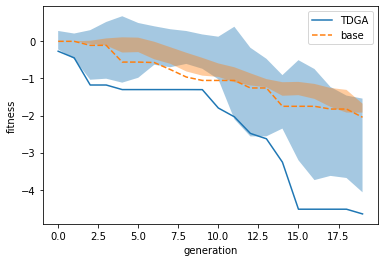
\includegraphics[clip,width=75mm]{fit.png}
    \caption{適応度の比較}
    \label{fig:fit}
  \end{center}
\end{figure}


図 \ref{fig:fit} に世代ごとの適応度の結果を示す.
折れ線が各世代の最良個体で, 領域が平均と標準偏差を示す.
最小化問題なので適応度は低いほうが良い.

多様性を示す $H$ をエントロピーから標準偏差に変えてみたが,
単純ながらも予想より優れた結果が出た.
多様性も選択の方法だけで常に確保できている事がわかった.

温度の設定は勘で決めたが, ここのパラメータ調整は難しそうな気がする.

\section{今後の予定}
% なんとなくなんかの勉強をするとかではなく具体的に

\begin{itemize}
  \item 個体の圧縮処理
  \item DARTSへの実装
\end{itemize}

% 参考文献リスト
\bibliographystyle{unsrt}
\bibliography{ref}
\end{document}
